\documentclass[8pt]{beamer}

\usetheme{metropolis}

\usepackage{pgfplots}
\usepackage{varwidth}
\usepackage{xcolor}

\usetikzlibrary{arrows}
\usetikzlibrary{arrows.meta}
\usetikzlibrary{calc}

\date{19.01.23}
\title{Introduction to Machine Learning}
\subtitle{Image recognition in Python and Tensorflow}
\author{Esten H. Leonardsen and Martin Hovin}

\titlegraphic{
	\centering
}

\colorlet{model1}{red}
\colorlet{model2}{green}
\colorlet{model3}{orange}

\def\nodesize{14pt}
\colorlet{nodefill}{green!20}

\begin{document}
	\begin{frame}
		\maketitle
	\end{frame}

	\begin{frame}{Introduction} % Speakers
		\centering
		\vfill
		\begin{tikzpicture}
			\node[] (esten) at (0, 0) {
				\includegraphics[width=2cm]{data/esten.jpg}
			};
			\node[] (martin) at (0, -3) {
				\includegraphics[width=2cm]{data/martin.png}
			};
			\node[align=left, anchor=west] at (esten.east) {
				\textbf{Esten H. Leonardsen}\\
				(UiO and Biometrical AS)\\
				\underline{Interests:}\\
				- Talking about esoteric theory\\
				- Making deep learning tutorials
			};
			\node[align=left, anchor=west] at (martin.east) {
				\textbf{Martin Hovin}\\
				(Biometrical AS)\\
				\underline{Interests:}\\
				- Installing tensorflow\\
				- Debugging Estens code
			};
		\end{tikzpicture}
		\vfill
	\end{frame}

	\begin{frame}{Introduction} % Learning goals
		\vfill
		Theory session:
		\begin{itemize}
			\item What is a statistical learning model?
			\item What is a loss function?
			\item How do we train a statistical learning model?
			\item How does a (deep) neural network work?
			\item What operations does a convolutional neural network use?
			\item What is transfer learning?
			\item What is overfitting?
			\item How do we combat it?
		\end{itemize}
		Practical session:
		\begin{enumerate}
			\item Set up a Python-environment containing Tensorflow
			\item Use a pretrained convolutional neural network to predict
			\item Fit a flower classifier using transfer learning
			\item Improve the flower classifier
		\end{enumerate}
		\vfill
	\end{frame}

	\begin{frame}{Introduction} % Motivation: Brain classification
	\end{frame}

	\begin{frame}{Introduction} % Motivation: Biometrical
	\end{frame}

	\begin{frame}{Introduction} % Motivation: Gjensidige
	\end{frame}

	\begin{frame}{Introduction} % Motivation: Segmentation
	\end{frame}

	\begin{frame}{Introduction} % Motivation: Imagen
		\centering
		\vfill
		\includegraphics[width=7cm]{data/dog-in-sushihouse.png}
		\vfill
	\end{frame}

	\begin{frame}{Statistical learning models} % Finn.no data
		\centering
		\vfill
		\begin{tikzpicture}
			\node[draw=black, inner sep=0pt] at (0, 0) {
				\includegraphics[height=7cm]{data/finn.png}
			};
		\end{tikzpicture}
		\vfill
	\end{frame}

	\begin{frame}{Statistical learning models} % Dataset
		\centering
		\vfill
		\begin{table}
			\begin{tabular}{|c|c|}
				\hline
				\textbf{$m^2$}&\textbf{Price}\\
				\hline
				72&5.127.379\\
				\hline
				50&4.552.170\\
				\hline
				45&4.486.654\\
				\hline
				62&5.709.276\\
				\hline
				53&4.634.912\\
				\hline
				81&8.388.570\\
				\hline
				44&4.828.170\\
				\hline
				78&7.557.770\\
				\hline
				37&4.016.520\\
				\hline
				73&6.572.351\\
				\hline
			\end{tabular}
		\end{table}
		\vfill
	\end{frame}

	\begin{frame}{Statistical learning models} % General Model
		\vfill
		\begin{tikzpicture}
			\begin{axis}[
				xlabel=$m^2$,
				ylabel=NOK,
				ytick={4000000, 5000000, 6000000, 7000000, 8000000},
				yticklabels={4M, 5M, 6M, 7M, 8M},
				scaled y ticks=false,
				xtick pos=bottom,
				ytick pos=left,
				xmin=30,
				xmax=90,,
				ymin=3500000,
				ymax=8800000
			]
				\addplot[
					only marks,
					mark size=3pt,
					mark options={draw=black, fill=cyan}
				] coordinates {
					(72, 5127379)
					(50, 4552170)
					(45, 4486654)
					(62, 5709276)
					(53, 4634912)
					(81, 8388570)
					(44, 4828170)
					(78, 7557770)
					(37, 4016520)
					(73, 6572351)
				};

				\newcommand{\loss}[2]{
					\addplot[dashed] coordinates {
						(####1, 3500000 + ####1 * 30000)
						(####1, ####2)
					};
				}

				\coordinate (center) at (axis cs: 60, 3500000);
			\end{axis}
			\node[anchor=north,align=center] (m1) at ($ (center) - (0, 1) $) {
				$\hat{y}=f(x)$
			};

			\node[] at ($ (center) - (5.3, 1.8) $) {};
			\node[] at ($ (center) + (5.3, 5.8) $) {};
		\end{tikzpicture}
		\vfill
	\end{frame}

	\begin{frame}{Statistical learning models} % Linear model
		\vfill
		\begin{tikzpicture}
			\begin{axis}[
				xlabel=$m^2$,
				ylabel=NOK,
				ytick={4000000, 5000000, 6000000, 7000000, 8000000},
				yticklabels={4M, 5M, 6M, 7M, 8M},
				scaled y ticks=false,
				xtick pos=bottom,
				ytick pos=left,
				xmin=30,
				xmax=90,,
				ymin=3500000,
				ymax=8800000
			]
				\addplot[
					only marks,
					mark size=3pt,
					mark options={draw=black, fill=cyan}
				] coordinates {
					(72, 5127379)
					(50, 4552170)
					(45, 4486654)
					(62, 5709276)
					(53, 4634912)
					(81, 8388570)
					(44, 4828170)
					(78, 7557770)
					(37, 4016520)
					(73, 6572351)
				};

				\newcommand{\loss}[2]{
					\addplot[dashed] coordinates {
						(####1, 3500000 + ####1 * 30000)
						(####1, ####2)
					};
				}

				\coordinate (center) at (axis cs: 60, 3500000);
			\end{axis}
			\node[anchor=north,align=center] (m1) at ($ (center) - (0, 1) $) {
				$\hat{y}=Wx+b$
			};

			\node[] at ($ (center) - (5.3, 1.8) $) {};
			\node[] at ($ (center) + (5.3, 5.8) $) {};
		\end{tikzpicture}
		\vfill
	\end{frame}

	\begin{frame}{Statistical learning models} % Concrete model
		\vfill
		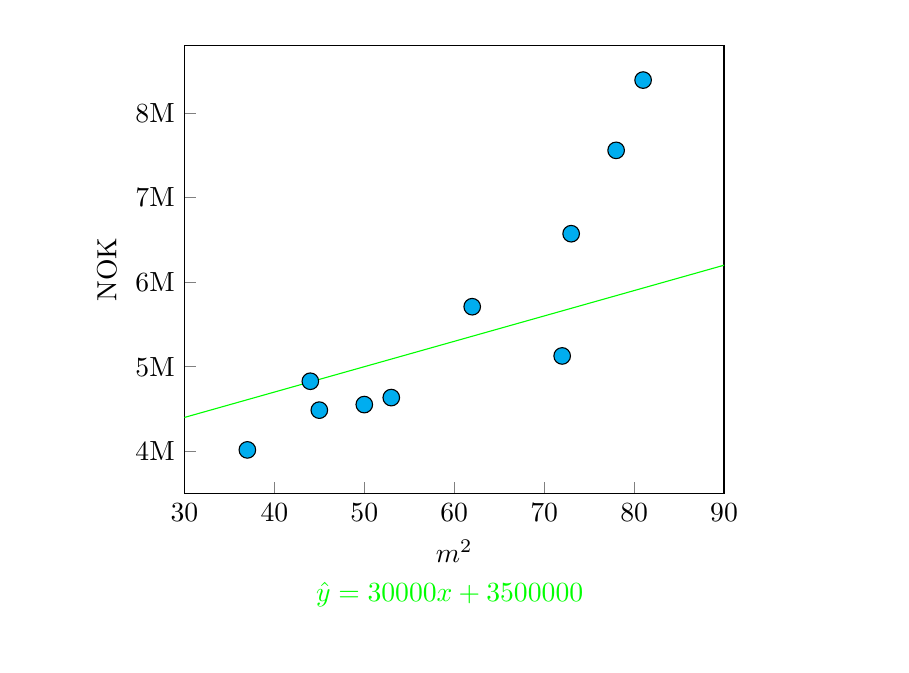
\begin{tikzpicture}
			\begin{axis}[
				xlabel=$m^2$,
				ylabel=NOK,
				ytick={4000000, 5000000, 6000000, 7000000, 8000000},
				yticklabels={4M, 5M, 6M, 7M, 8M},
				scaled y ticks=false,
				xtick pos=bottom,
				ytick pos=left,
				xmin=30,
				xmax=90,,
				ymin=3500000,
				ymax=8800000
			]
				\addplot[
					only marks,
					mark size=3pt,
					mark options={draw=black, fill=cyan}
				] coordinates {
					(72, 5127379)
					(50, 4552170)
					(45, 4486654)
					(62, 5709276)
					(53, 4634912)
					(81, 8388570)
					(44, 4828170)
					(78, 7557770)
					(37, 4016520)
					(73, 6572351)
				};
				\addplot[model2] coordinates {
					(0, 3500000)
					(100, 6500000)
				};

				\newcommand{\loss}[2]{
					\addplot[dashed] coordinates {
						(####1, 3500000 + ####1 * 30000)
						(####1, ####2)
					};
				}

				\coordinate (center) at (axis cs: 60, 3500000);
			\end{axis}
			\node[anchor=north,align=center, text=model2] (m1) at ($ (center) - (0, 1) $) {
				$\hat{y}=30000x + 3500000$
			};

			\node[] at ($ (center) - (5.3, 1.8) $) {};
			\node[] at ($ (center) + (5.3, 5.8) $) {};
		\end{tikzpicture}
		\vfill
	\end{frame}

	\begin{frame}{Statistical learning models} % Alternative models
		\vfill
		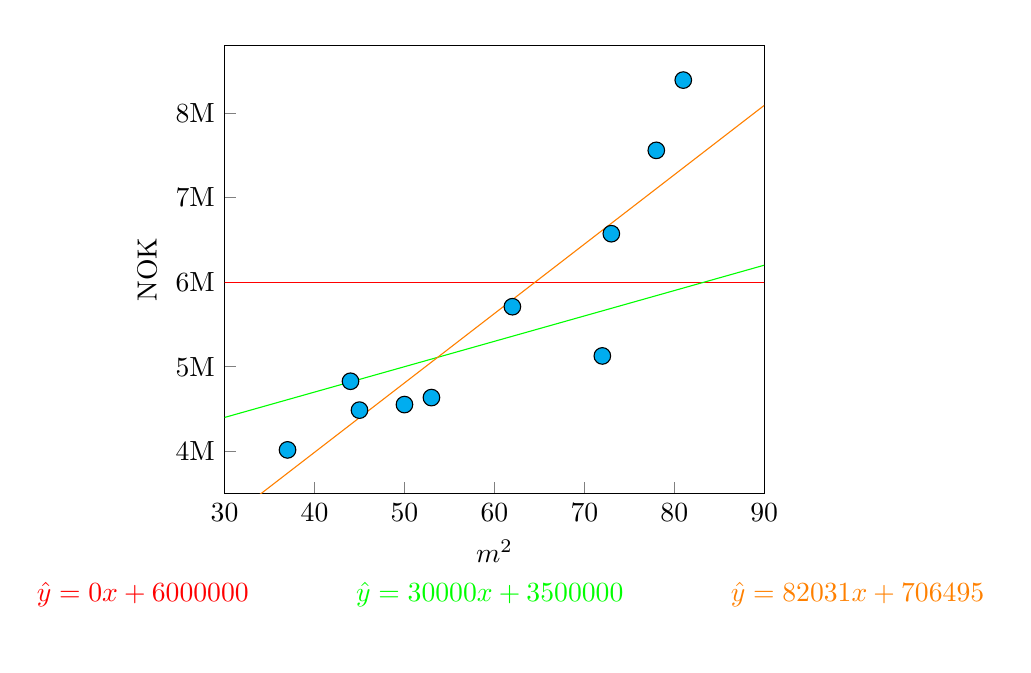
\begin{tikzpicture}
			\begin{axis}[
				xlabel=$m^2$,
				ylabel=NOK,
				ytick={4000000, 5000000, 6000000, 7000000, 8000000},
				yticklabels={4M, 5M, 6M, 7M, 8M},
				scaled y ticks=false,
				xtick pos=bottom,
				ytick pos=left,
				xmin=30,
				xmax=90,,
				ymin=3500000,
				ymax=8800000
			]
				\addplot[
					only marks,
					mark size=3pt,
					mark options={draw=black, fill=cyan}
				] coordinates {
					(72, 5127379)
					(50, 4552170)
					(45, 4486654)
					(62, 5709276)
					(53, 4634912)
					(81, 8388570)
					(44, 4828170)
					(78, 7557770)
					(37, 4016520)
					(73, 6572351)
				};
				\addplot[model1] coordinates {
					(0, 6000000)
					(100, 6000000)
				};
				\addplot[model2] coordinates {
					(0, 3500000)
					(100, 6500000)
				};
				\addplot[model3] coordinates {
					(0, 706495)
					(100, 8909658)
				};

				\newcommand{\loss}[2]{
					\addplot[dashed] coordinates {
						(####1, 3500000 + ####1 * 30000)
						(####1, ####2)
					};
				}

				\coordinate (center) at (axis cs: 60, 3500000);
			\end{axis}
			\node[anchor=north,align=center, text=model2] (m1) at ($ (center) - (0, 1) $) {
				$\hat{y}=30000x + 3500000$
			};

			\node[anchor=east,align=center, text=model1] at ($ (m1.west) + (-1, 0) $) {
				$\hat{y}=0x + 6000000$
			};

			\node[anchor=west,align=center, text=model3] at ($ (m1.east) + (1, 0) $) {
				$\hat{y}=82031x + 706495$
			};

			\node[] at ($ (center) - (5.3, 1.8) $) {};
			\node[] at ($ (center) + (5.3, 5.8) $) {};
		\end{tikzpicture}
		\vfill
	\end{frame}

	\begin{frame}{Loss functions} % Model
		\vfill
		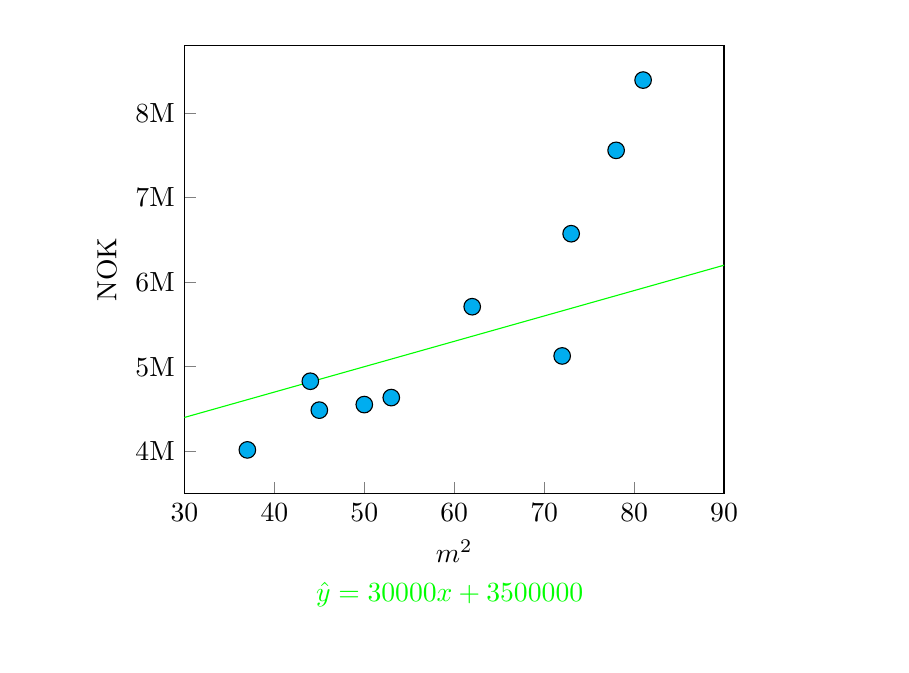
\begin{tikzpicture}
			\begin{axis}[
				xlabel=$m^2$,
				ylabel=NOK,
				ytick={4000000, 5000000, 6000000, 7000000, 8000000},
				yticklabels={4M, 5M, 6M, 7M, 8M},
				scaled y ticks=false,
				xtick pos=bottom,
				ytick pos=left,
				xmin=30,
				xmax=90,,
				ymin=3500000,
				ymax=8800000
			]
				\addplot[
					only marks,
					mark size=3pt,
					mark options={draw=black, fill=cyan}
				] coordinates {
					(72, 5127379)
					(50, 4552170)
					(45, 4486654)
					(62, 5709276)
					(53, 4634912)
					(81, 8388570)
					(44, 4828170)
					(78, 7557770)
					(37, 4016520)
					(73, 6572351)
				};
				\addplot[model2] coordinates {
					(0, 3500000)
					(100, 6500000)
				};

				\newcommand{\loss}[2]{
					\addplot[dashed] coordinates {
						(####1, 3500000 + ####1 * 30000)
						(####1, ####2)
					};
				}

				\coordinate (center) at (axis cs: 60, 3500000);
			\end{axis}
			\node[anchor=north,align=center, text=model2] (m1) at ($ (center) - (0, 1) $) {
				$\hat{y}=30000x + 3500000$
			};

			\node[] at ($ (center) - (5.3, 1.8) $) {};
			\node[] at ($ (center) + (5.3, 5.8) $) {};
		\end{tikzpicture}
		\vfill
	\end{frame}

	\begin{frame}{Loss functions} % Prediction
		\vfill
		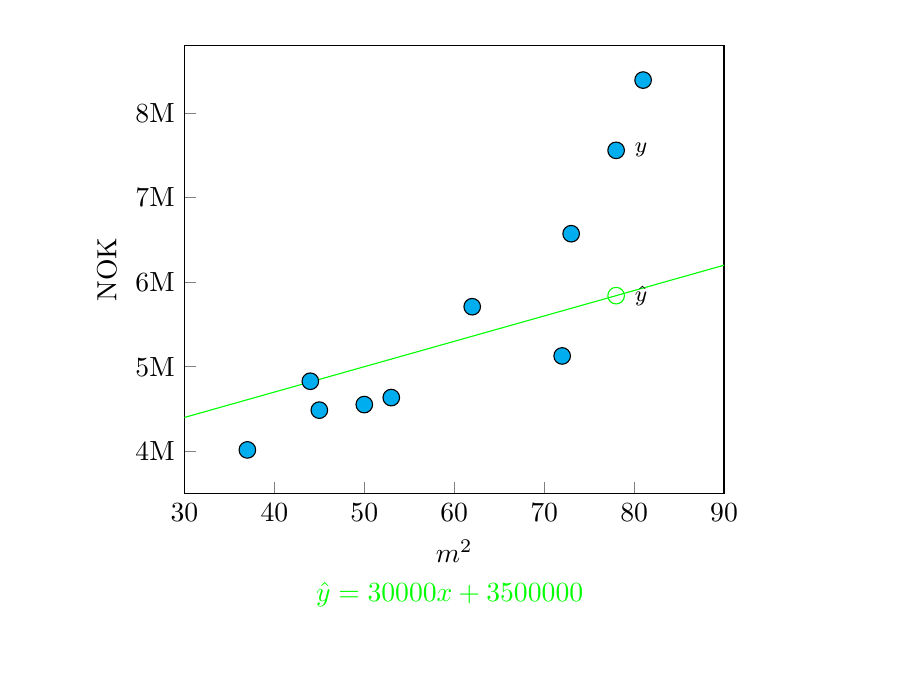
\begin{tikzpicture}
			\begin{axis}[
				xlabel=$m^2$,
				ylabel=NOK,
				ytick={4000000, 5000000, 6000000, 7000000, 8000000},
				yticklabels={4M, 5M, 6M, 7M, 8M},
				scaled y ticks=false,
				xtick pos=bottom,
				ytick pos=left,
				xmin=30,
				xmax=90,,
				ymin=3500000,
				ymax=8800000
			]
				\addplot[
					only marks,
					mark size=3pt,
					mark options={draw=black, fill=cyan}
				] coordinates {
					(72, 5127379)
					(50, 4552170)
					(45, 4486654)
					(62, 5709276)
					(53, 4634912)
					(81, 8388570)
					(44, 4828170)
					(78, 7557770)
					(37, 4016520)
					(73, 6572351)
				};
				\addplot[
					only marks,
					mark size=3pt,
					mark options={draw=green, fill=white},
					fill opacity=0
				] coordinates {
					(78, 3500000 + 78 * 30000)
				};
				\addplot[model2] coordinates {
					(0, 3500000)
					(100, 6500000)
				};

				\newcommand{\loss}[2]{
					\addplot[dashed] coordinates {
						(####1, 3500000 + ####1 * 30000)
						(####1, ####2)
					};
				}

				\coordinate (center) at (axis cs: 60, 3500000);
				\node[anchor=west] at (axis cs: 79, 5840000) {\footnotesize{$\hat{y}$}};
				\node[anchor=west] at (axis cs: 79, 7557770) {\footnotesize{$y$}};
			\end{axis}
			\node[anchor=north,align=center, text=model2] (m1) at ($ (center) - (0, 1) $) {
				$\hat{y}=30000x + 3500000$
			};

			\node[] at ($ (center) - (5.3, 1.8) $) {};
			\node[] at ($ (center) + (5.3, 5.8) $) {};
		\end{tikzpicture}
		\vfill
	\end{frame}

	\begin{frame}{Loss functions} % Squared error
		\vfill
		\begin{tikzpicture}
			\begin{axis}[
				xlabel=$m^2$,
				ylabel=NOK,
				ytick={4000000, 5000000, 6000000, 7000000, 8000000},
				yticklabels={4M, 5M, 6M, 7M, 8M},
				scaled y ticks=false,
				xtick pos=bottom,
				ytick pos=left,
				xmin=30,
				xmax=90,,
				ymin=3500000,
				ymax=8800000
			]
				\addplot[
					only marks,
					mark size=3pt,
					mark options={draw=black, fill=cyan}
				] coordinates {
					(72, 5127379)
					(50, 4552170)
					(45, 4486654)
					(62, 5709276)
					(53, 4634912)
					(81, 8388570)
					(44, 4828170)
					(78, 7557770)
					(37, 4016520)
					(73, 6572351)
				};
				\addplot[
					only marks,
					mark size=3pt,
					mark options={draw=green, fill=white},
					fill opacity=0
				] coordinates {
					(78, 3500000 + 78 * 30000)
				};
				\addplot[model2] coordinates {
					(0, 3500000)
					(100, 6500000)
				};

				\newcommand{\loss}[2]{
					\addplot[dashed] coordinates {
						(####1, 3500000 + ####1 * 30000)
						(####1, ####2)
					};
				}

				\loss{78}{7557770}

				\coordinate (center) at (axis cs: 60, 3500000);
				\node[anchor=west] at (axis cs: 79, 5840000) {\footnotesize{$\hat{y}$}};
				\node[anchor=west] at (axis cs: 79, 7557770) {\footnotesize{$y$}};
				\node[anchor=west] at (axis cs: 78, 6698885) {\footnotesize{$\ell=(y-\hat{y})^2$}};
			\end{axis}
			\node[anchor=north,align=center, text=model2] (m1) at ($ (center) - (0, 1) $) {
				$\hat{y}=30000x + 3500000$
			};

			\node[] at ($ (center) - (5.3, 1.8) $) {};
			\node[] at ($ (center) + (5.3, 5.8) $) {};
		\end{tikzpicture}
		\vfill
	\end{frame}

	\begin{frame}{Loss functions} % Mean squared error
		\vfill
		\begin{tikzpicture}
			\begin{axis}[
				xlabel=$m^2$,
				ylabel=NOK,
				ytick={4000000, 5000000, 6000000, 7000000, 8000000},
				yticklabels={4M, 5M, 6M, 7M, 8M},
				scaled y ticks=false,
				xtick pos=bottom,
				ytick pos=left,
				xmin=30,
				xmax=90,,
				ymin=3500000,
				ymax=8800000
			]
				\addplot[
					only marks,
					mark size=3pt,
					mark options={draw=black, fill=cyan}
				] coordinates {
					(72, 5127379)
					(50, 4552170)
					(45, 4486654)
					(62, 5709276)
					(53, 4634912)
					(81, 8388570)
					(44, 4828170)
					(78, 7557770)
					(37, 4016520)
					(73, 6572351)
				};
				\addplot[
					only marks,
					mark size=3pt,
					mark options={draw=green, fill=white},
					fill opacity=0
				] coordinates {
					(72, 3500000 + 72 * 30000)
					(50, 3500000 + 50 * 30000)
					(45, 3500000 + 45 * 30000)
					(62, 3500000 + 62 * 30000)
					(53, 3500000 + 53 * 30000)
					(81, 3500000 + 81 * 30000)
					(44, 3500000 + 44 * 30000)
					(78, 3500000 + 78 * 30000)
					(37, 3500000 + 37 * 30000)
					(73, 3500000 + 73 * 30000)
				};
				\addplot[model2] coordinates {
					(0, 3500000)
					(100, 6500000)
				};

				\newcommand{\loss}[2]{
					\addplot[dashed] coordinates {
						(####1, 3500000 + ####1 * 30000)
						(####1, ####2)
					};
				}

				\loss{72}{5127379}
				\loss{50}{4552170}
				\loss{45}{4486654}
				\loss{62}{5709276}
				\loss{53}{4634912}
				\loss{81}{8388570}
				\loss{44}{4828170}
				\loss{78}{7557770}
				\loss{37}{4016520}
				\loss{73}{6572351}

				\coordinate (center) at (axis cs: 60, 3500000);
			\end{axis}
			\node[anchor=north,align=center, text=model2] (m1) at ($ (center) - (0, 1) $) {
				$\hat{y}=30000x + 3500000$\\
				$\ell=\sum (y - \hat{y})^2$
			};

			\node[] at ($ (center) - (5.3, 1.8) $) {};
			\node[] at ($ (center) + (5.3, 5.8) $) {};
		\end{tikzpicture}
		\vfill
	\end{frame}

	\begin{frame}{Loss functions} % Loss computation
		\vfill
		\begin{tikzpicture}
			\begin{axis}[
				xlabel=$m^2$,
				ylabel=NOK,
				ytick={4000000, 5000000, 6000000, 7000000, 8000000},
				yticklabels={4M, 5M, 6M, 7M, 8M},
				scaled y ticks=false,
				xtick pos=bottom,
				ytick pos=left,
				xmin=30,
				xmax=90,,
				ymin=3500000,
				ymax=8800000
			]
				\addplot[
					only marks,
					mark size=3pt,
					mark options={draw=black, fill=cyan}
				] coordinates {
					(72, 5127379)
					(50, 4552170)
					(45, 4486654)
					(62, 5709276)
					(53, 4634912)
					(81, 8388570)
					(44, 4828170)
					(78, 7557770)
					(37, 4016520)
					(73, 6572351)
				};
				\addplot[
					only marks,
					mark size=3pt,
					mark options={draw=green, fill=white},
					fill opacity=0
				] coordinates {
					(72, 3500000 + 72 * 30000)
					(50, 3500000 + 50 * 30000)
					(45, 3500000 + 45 * 30000)
					(62, 3500000 + 62 * 30000)
					(53, 3500000 + 53 * 30000)
					(81, 3500000 + 81 * 30000)
					(44, 3500000 + 44 * 30000)
					(78, 3500000 + 78 * 30000)
					(37, 3500000 + 37 * 30000)
					(73, 3500000 + 73 * 30000)
				};
				\addplot[model2] coordinates {
					(0, 3500000)
					(100, 6500000)
				};

				\newcommand{\loss}[2]{
					\addplot[dashed] coordinates {
						(####1, 3500000 + ####1 * 30000)
						(####1, ####2)
					};
				}

				\loss{72}{5127379}
				\loss{50}{4552170}
				\loss{45}{4486654}
				\loss{62}{5709276}
				\loss{53}{4634912}
				\loss{81}{8388570}
				\loss{44}{4828170}
				\loss{78}{7557770}
				\loss{37}{4016520}
				\loss{73}{6572351}

				\coordinate (center) at (axis cs: 60, 3500000);
			\end{axis}
			\node[anchor=north,align=center, text=model2] (m1) at ($ (center) - (0, 1) $) {
				$\hat{y}=30000x + 3500000$\\
				$\ell=1.10 \times 10^{13}$
			};

			\node[] at ($ (center) - (5.3, 1.8) $) {};
			\node[] at ($ (center) + (5.3, 5.8) $) {};
		\end{tikzpicture}
		\vfill
	\end{frame}

	\begin{frame}{Loss functions} % Loss comparison
		\vfill
		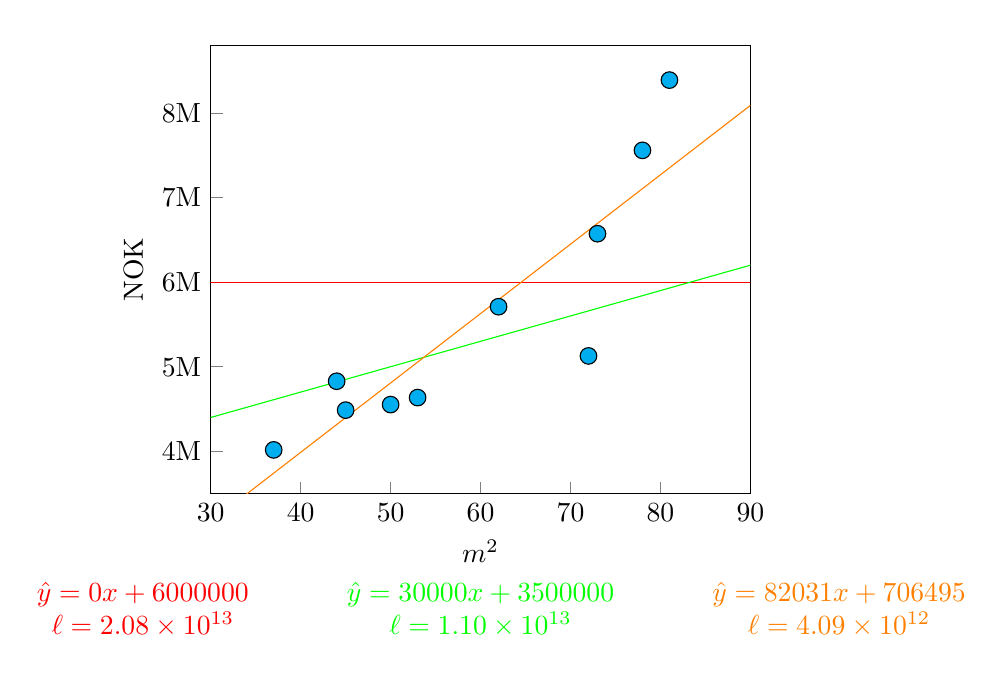
\begin{tikzpicture}
			\begin{axis}[
				xlabel=$m^2$,
				ylabel=NOK,
				ytick={4000000, 5000000, 6000000, 7000000, 8000000},
				yticklabels={4M, 5M, 6M, 7M, 8M},
				scaled y ticks=false,
				xtick pos=bottom,
				ytick pos=left,
				xmin=30,
				xmax=90,,
				ymin=3500000,
				ymax=8800000
			]
				\addplot[
					only marks,
					mark size=3pt,
					mark options={draw=black, fill=cyan}
				] coordinates {
					(72, 5127379)
					(50, 4552170)
					(45, 4486654)
					(62, 5709276)
					(53, 4634912)
					(81, 8388570)
					(44, 4828170)
					(78, 7557770)
					(37, 4016520)
					(73, 6572351)
				};
				\addplot[model1] coordinates {
					(0, 6000000)
					(100, 6000000)
				};
				\addplot[model2] coordinates {
					(0, 3500000)
					(100, 6500000)
				};
				\addplot[model3] coordinates {
					(0, 706495)
					(100, 8909658)
				};
				\coordinate (center) at (axis cs: 60, 3500000);
			\end{axis}
			\node[anchor=north,align=center, text=model2] (m1) at ($ (center) - (0, 1) $) {
				$\hat{y}=30000x + 3500000$\\
				$\ell=1.10 \times 10^{13}$
			};


			\node[anchor=east,align=center, text=model1] at ($ (m1.west) + (-1, 0) $) {
				$\hat{y}=0x + 6000000$\\
				$\ell=2.08 \times 10^{13}$
			};

			\node[anchor=west,align=center, text=model3] at ($ (m1.east) + (1, 0) $) {
				$\hat{y}=82031x + 706495$\\
				$\ell=4.09 \times 10^{12}$
			};

			\node[] at ($ (center) - (5.3, 1.8) $) {};
			\node[] at ($ (center) + (5.3, 5.8) $) {};
		\end{tikzpicture}
		\vfill
	\end{frame}

	\begin{frame}{Training} % Formulas
		\vfill
		\begin{tikzpicture}
			\begin{axis}[
				xlabel=$m^2$,
				ylabel=NOK,
				ytick={4000000, 5000000, 6000000, 7000000, 8000000},
				yticklabels={4M, 5M, 6M, 7M, 8M},
				scaled y ticks=false,
				xtick pos=bottom,
				ytick pos=left,
				xmin=30,
				xmax=90,,
				ymin=3500000,
				ymax=8800000
			]
				\addplot[
					only marks,
					mark size=3pt,
					mark options={draw=black, fill=cyan}
				] coordinates {
					(72, 5127379)
					(50, 4552170)
					(45, 4486654)
					(62, 5709276)
					(53, 4634912)
					(81, 8388570)
					(44, 4828170)
					(78, 7557770)
					(37, 4016520)
					(73, 6572351)
				};
				\addplot[model2] coordinates {
					(0, 3500000)
					(100, 6500000)
				};
				\coordinate (center) at (axis cs: 60, 3500000);
			\end{axis}
			\node[anchor=north,align=center] (m1) at ($ (center) - (0, 1) $) {
				$\hat{y}=Wx + b$\\
				$\ell=\sum (y - \hat{y})^2$
			};

			\node[] at ($ (center) - (5.3, 1.8) $) {};
			\node[] at ($ (center) + (5.3, 5.8) $) {};
		\end{tikzpicture}
		\vfill
	\end{frame}

	\begin{frame}{Training} % Formula replacement
		\vfill
		\begin{tikzpicture}
			\begin{axis}[
				xlabel=$m^2$,
				ylabel=NOK,
				ytick={4000000, 5000000, 6000000, 7000000, 8000000},
				yticklabels={4M, 5M, 6M, 7M, 8M},
				scaled y ticks=false,
				xtick pos=bottom,
				ytick pos=left,
				xmin=30,
				xmax=90,,
				ymin=3500000,
				ymax=8800000
			]
				\addplot[
					only marks,
					mark size=3pt,
					mark options={draw=black, fill=cyan}
				] coordinates {
					(72, 5127379)
					(50, 4552170)
					(45, 4486654)
					(62, 5709276)
					(53, 4634912)
					(81, 8388570)
					(44, 4828170)
					(78, 7557770)
					(37, 4016520)
					(73, 6572351)
				};
				\addplot[model2] coordinates {
					(0, 3500000)
					(100, 6500000)
				};
				\coordinate (center) at (axis cs: 60, 3500000);
			\end{axis}


			\node[anchor=north,align=center] (m1) at ($ (center) - (0, 1) $) {
				$\hat{y}=Wx + b$\\
				$\ell=\sum (y - \hat{y})^2$
			};
			\node[
				draw=red,
				anchor=north west,
				minimum height=0.4cm,
				minimum width=0.3cm
			] at ($ (m1.north west) + (0.21, -0.03) $) {};
			\node[
				draw=red,
				anchor=south east,
				minimum height=0.4cm,
				minimum width=0.3cm
			] at ($ (m1.south east) + (-0.27, 0.05) $) {};

			\node[] at ($ (center) - (5.3, 1.8) $) {};
			\node[] at ($ (center) + (5.3, 5.8) $) {};
		\end{tikzpicture}
		\vfill
	\end{frame}

	\begin{frame}{Training} % Single formula
		\vfill
		\begin{tikzpicture}
			\begin{axis}[
				xlabel=$m^2$,
				ylabel=NOK,
				ytick={4000000, 5000000, 6000000, 7000000, 8000000},
				yticklabels={4M, 5M, 6M, 7M, 8M},
				scaled y ticks=false,
				xtick pos=bottom,
				ytick pos=left,
				xmin=30,
				xmax=90,,
				ymin=3500000,
				ymax=8800000
			]
				\addplot[
					only marks,
					mark size=3pt,
					mark options={draw=black, fill=cyan}
				] coordinates {
					(72, 5127379)
					(50, 4552170)
					(45, 4486654)
					(62, 5709276)
					(53, 4634912)
					(81, 8388570)
					(44, 4828170)
					(78, 7557770)
					(37, 4016520)
					(73, 6572351)
				};
				\addplot[model2] coordinates {
					(0, 3500000)
					(100, 6500000)
				};
				\coordinate (center) at (axis cs: 60, 3500000);
			\end{axis}


			\node[anchor=north,align=center] (m1) at ($ (center) - (0, 1) $) {
				$\ell=\sum (y - (Wx + b))^2$
			};

			\node[] at ($ (center) - (5.3, 1.8) $) {};
			\node[] at ($ (center) + (5.3, 5.8) $) {};
		\end{tikzpicture}
		\vfill
	\end{frame}

	\begin{frame}{Training} % Actual formula
		\vfill
		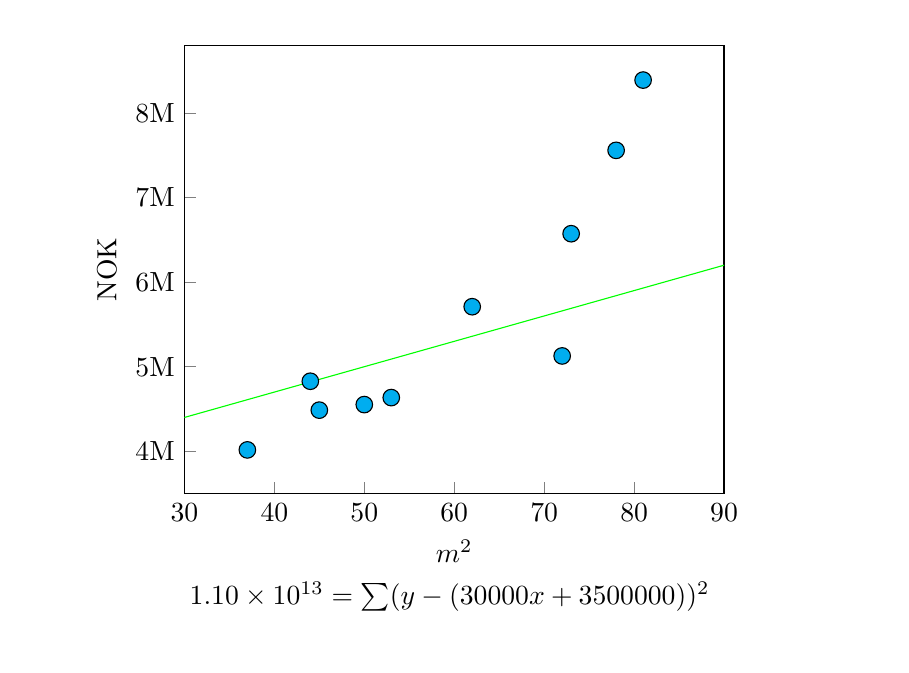
\begin{tikzpicture}
			\begin{axis}[
				xlabel=$m^2$,
				ylabel=NOK,
				ytick={4000000, 5000000, 6000000, 7000000, 8000000},
				yticklabels={4M, 5M, 6M, 7M, 8M},
				scaled y ticks=false,
				xtick pos=bottom,
				ytick pos=left,
				xmin=30,
				xmax=90,,
				ymin=3500000,
				ymax=8800000
			]
				\addplot[
					only marks,
					mark size=3pt,
					mark options={draw=black, fill=cyan}
				] coordinates {
					(72, 5127379)
					(50, 4552170)
					(45, 4486654)
					(62, 5709276)
					(53, 4634912)
					(81, 8388570)
					(44, 4828170)
					(78, 7557770)
					(37, 4016520)
					(73, 6572351)
				};
				\addplot[model2] coordinates {
					(0, 3500000)
					(100, 6500000)
				};
				\coordinate (center) at (axis cs: 60, 3500000);
			\end{axis}


			\node[anchor=north,align=center] (m1) at ($ (center) - (0, 1) $) {
				$1.10 \times 10^{13}=\sum (y - (30000x + 3500000))^2$
			};

			\node[] at ($ (center) - (5.3, 1.8) $) {};
			\node[] at ($ (center) + (5.3, 5.8) $) {};
		\end{tikzpicture}
		\vfill
	\end{frame}

	\begin{frame}{Training} % Update
		\vfill
		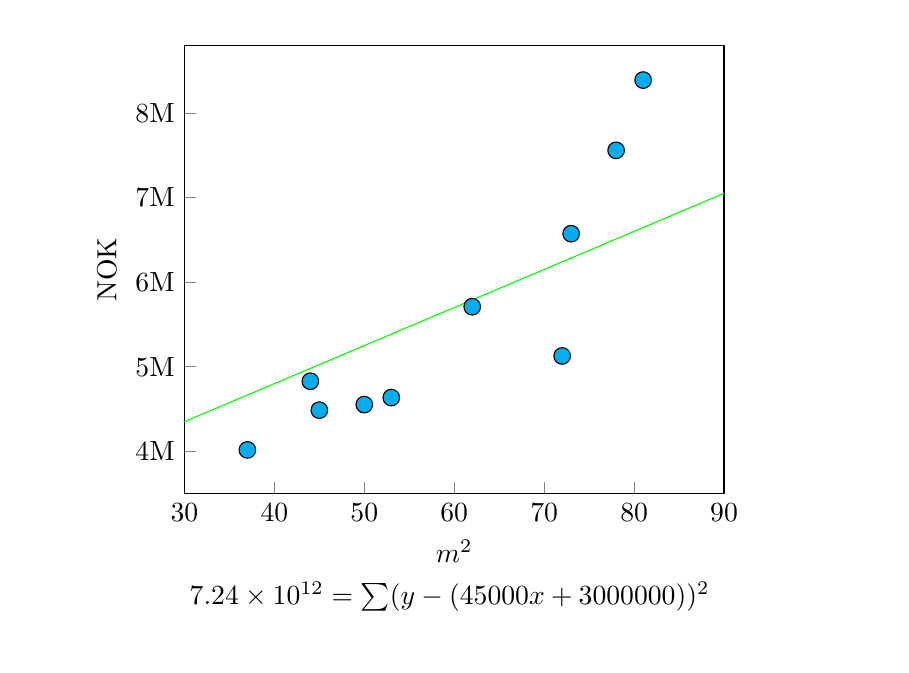
\begin{tikzpicture}
			\begin{axis}[
				xlabel=$m^2$,
				ylabel=NOK,
				ytick={4000000, 5000000, 6000000, 7000000, 8000000},
				yticklabels={4M, 5M, 6M, 7M, 8M},
				scaled y ticks=false,
				xtick pos=bottom,
				ytick pos=left,
				xmin=30,
				xmax=90,,
				ymin=3500000,
				ymax=8800000
			]
				\addplot[
					only marks,
					mark size=3pt,
					mark options={draw=black, fill=cyan}
				] coordinates {
					(72, 5127379)
					(50, 4552170)
					(45, 4486654)
					(62, 5709276)
					(53, 4634912)
					(81, 8388570)
					(44, 4828170)
					(78, 7557770)
					(37, 4016520)
					(73, 6572351)
				};
				\addplot[model2] coordinates {
					(0, 3000000)
					(100, 7500000)
				};
				\coordinate (center) at (axis cs: 60, 3500000);
			\end{axis}


			\node[anchor=north,align=center] (m1) at ($ (center) - (0, 1) $) {
				$7.24 \times 10^{12}=\sum (y - (45000x + 3000000))^2$
			};

			\node[] at ($ (center) - (5.3, 1.8) $) {};
			\node[] at ($ (center) + (5.3, 5.8) $) {};
		\end{tikzpicture}
		\vfill
	\end{frame}

	\begin{frame}{Building a neural network} % Linear regression
		\centering
		\vfill
		\begin{tikzpicture}
			\node[] at (-5, 3) {};
			\node[] at (5, -4.5) {};

			\node[
				circle,
				draw=black,
				fill=nodefill,
				minimum size=\nodesize,
				inner sep=0pt
			] (n) at (0, 1.5) {};
			\node[] (x) at (-1.5, 1.5) {$x$};
			\node[] (b) at (0, 2.5) {$b$};
			\node[] (y) at (1.5, 1.5) {$y$};
			\node[] at (0, 0) {$\hat{y}=wx+b$};

			\draw[->] (x) -- (n) node [midway, above] {$w$};
			\draw[->] (b) -- (n);
			\draw[->] (n) -- (y);
		\end{tikzpicture}
		\vfill
	\end{frame}

	\begin{frame}{Building a neural network} % Straight line
		\centering
		\vfill
		\begin{tikzpicture}
			\node[] at (-5, 3) {};
			\node[] at (5, -4.5) {};

			\node[
				circle,
				draw=black,
				fill=nodefill,
				minimum size=\nodesize,
				inner sep=0pt
			] (n) at (0, 1.5) {};
			\node[] (x) at (-1.5, 1.5) {$x$};
			\node[] (b) at (0, 2.5) {$b$};
			\node[] (y) at (1.5, 1.5) {$y$};
			\node[] at (0, 0) {$\hat{y}=wx+b$};

			\draw[->] (x) -- (n) node [midway, above] {$w$};
			\draw[->] (b) -- (n);
			\draw[->] (n) -- (y);

			\draw[] (-2, -1.5) -- (2, -1.5) -- (2, -4) -- (-2, -4) -- (-2, -1.5);

			\draw[very thick, blue!60] (-2, -3.5) -- (2, -1.75);

			\node[anchor=north] at (0, -4.1) {x};
			\node[anchor=south, rotate=90] at (-2.1, -2.75) {y};
		\end{tikzpicture}
		\vfill
	\end{frame}

	\begin{frame}{Building a neural network} % Non-linearity
		\centering
		\vfill
		\begin{tikzpicture}
			\node[] at (-5, 3) {};
			\node[] at (5, -4.5) {};

			\node[
				circle,
				draw=black,
				fill=nodefill,
				minimum size=\nodesize,
				inner sep=0pt
			] (n) at (0, 1.5) {};
			\node[] (x) at (-1.5, 1.5) {$x$};
			\node[] (b) at (0, 2.5) {$b$};
			\node[] (y) at (1.5, 1.5) {$y$};
			\node[] at (0, 0) {$\hat{y}=max(0, wx+b)$};

			\draw[->] (x) -- (n) node [midway, above] {$w$};
			\draw[->] (b) -- (n);
			\draw[->] (n) -- (y);

			\draw[] (-2, -1.5) -- (2, -1.5) -- (2, -4) -- (-2, -4) -- (-2, -1.5);
			\draw[very thick, blue!60] (-2, -3.5) -- (0, -3.5) -- (2, -1.75);

			\node[anchor=north] at (0, -4.1) {x};
			\node[anchor=south, rotate=90] at (-2.1, -2.75) {y};
		\end{tikzpicture}
		\vfill
	\end{frame}

	\begin{frame}{Building a neural network} % MLP
		\centering
		\vfill
		\begin{tikzpicture}
			\node[] at (-5, 3) {};
			\node[] at (5, -4.5) {};

			\node[
				circle,
				draw=black,
				fill=green!20,
				minimum size=\nodesize,
				inner sep=0pt
			] (n0) at (0, 2) {};
			\node[
				circle,
				draw=black,
				fill=nodefill,
				minimum size=\nodesize,
				inner sep=0pt
			] (n1) at (0, 1) {};
			\node[] (x) at (-1.5, 1.5) {$x$};
			\node[] (y) at (1.5, 1.5) {$y$};
			\node[] at (0, 0) {$\hat{y}=max(0, w_0x+b_0)+max(0, w_1x+b_1)$};

			\draw[->] (x) -- (n0) node [midway, above] {$w_0$};
			\draw[->] (x) -- (n1) node [midway, below] {$w_1$};
			\draw[->] (n0) -- (y);
			\draw[->] (n1) -- (y);

			\draw[] (-2, -1.5) -- (2, -1.5) -- (2, -4) -- (-2, -4) -- (-2, -1.5);
			\draw[very thick, blue!60] (-2, -3.5) -- (-0.66, -3.5) -- (0.66, -2.25) -- (2, -3);

			\node[anchor=north] at (0, -4.1) {x};
			\node[anchor=south, rotate=90] at (-2.1, -2.75) {y};
		\end{tikzpicture}
		\vfill
	\end{frame}

	\begin{frame}{Building a neural network} % Universal approximation theorem
		\vfill
		\centering
		\begin{quotation}
			\centering
			"Any relationship that can be described with a polynomial function can be approximated by a neural network with a single hidden layer."
		\end{quotation}
		\vfill
	\end{frame}

	\begin{frame}{Building a neural network} % Multidimensional
		\centering
		\vfill
		\newsavebox{\mybox}
		\sbox{\mybox}{%
			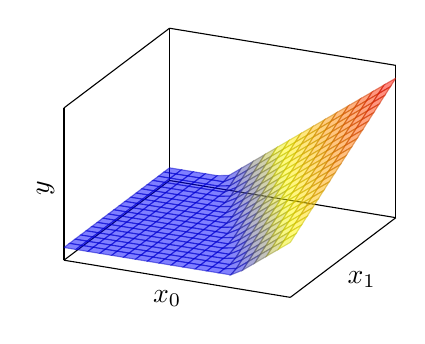
\begin{tikzpicture}[
				declare function = {
					q(\x) = \x - 1;
					Z(\x,\y) = max(0, \x*0.5 + \y*0.25);
				}
			]
				\begin{axis}
				[
					height=5cm,
					ticks=none,
					xlabel=$x_0$,
					ylabel=$x_1$,
					zlabel=$y$,
					domain=-1:1,
					samples=20,
				]
					\addplot3 [surf, opacity=0.5] {Z(x,y)};
				\end{axis}
			\end{tikzpicture}
		}
		\begin{tikzpicture}
			\node[] at (-5, 3) {};
			\node[] at (5, -4.5) {};

			\node[
				circle,
				draw=black,
				fill=nodefill,
				minimum size=\nodesize,
				inner sep=0pt
			] (n) at (0, 1.5) {};
			\node[] (x0) at (-1.5, 2) {$x_0$};
			\node[] (x1) at (-1.5, 1) {$x_1$};
			\node[] (b) at (0, 2.5) {$b$};
			\node[] (y) at (1.5, 1.5) {$y$};
			\node[] at (0, 0) {$\hat{y}=max(0, w_0x_0+w_1x_1+b)$};

			\draw[->] (x0) -- (n) node [midway, above] {$w_0$};
			\draw[->] (x1) -- (n) node [midway, below] {$w_1$};
			\draw[->] (b) -- (n);
			\draw[->] (n) -- (y);

			\node[] at (0, -2.75) {
				\usebox{\mybox}
			};
		\end{tikzpicture}
		\vfill
	\end{frame}

	\begin{frame}{Building a neural network} % Actual MLP
		\centering
		\vfill
		\begin{tikzpicture}
			\node[] at (-3.5, 1.25) {};
			\node[] at (3.5, -6.25) {};
			\node[
				circle,
				minimum size=\nodesize,
				inner sep=0pt,
				text depth=0
			] (x) at (-3, 0) {\footnotesize{$x$}};

			\node[
				circle,
				draw=black,
				fill=nodefill,
				minimum size=\nodesize,
				inner sep=0pt
			] (n00) at (0, 0.5) {};
			\node[
				circle,
				draw=black,
				fill=nodefill,
				minimum size=\nodesize,
				inner sep=0pt
			] (n01) at (0, -0.5) {};

			\node[
				circle,
				minimum size=\nodesize,
				inner sep=0pt,
				text depth=0
			] (y) at (3, 0) {\footnotesize{$y$}};

			\draw[->] (x) -- (n00) node [midway, above] {$w_0$};
			\draw[->] (x) -- (n01) node [midway, below] {$w_1$};

			\draw[->] (n00) -- (y);
			\draw[->] (n01) -- (y);

			\def\spacing{-0.1cm}
			\node[anchor=north] at (0, -1.5) {\tiny{
				\begin{math}
					\begin{alignedat}{5}
						\hat{y} = max(0, w_0x+b_0)+max(0, w_1x+b_1)\\
					\end{alignedat}
				\end{math}
			}};
		\end{tikzpicture}
		\vfill
	\end{frame}

	\begin{frame}{Building a neural network} % Input/output layers
		\centering
		\vfill
		\begin{tikzpicture}
			\node[] at (-3.5, 1.25) {};
			\node[] at (3.5, -6.25) {};
			\node[
				circle,
				draw=black,
				fill=nodefill,
				minimum size=\nodesize,
				inner sep=0pt,
				text depth=0
			] (x) at (-3, 0) {\footnotesize{$x$}};

			\node[
				circle,
				draw=black,
				fill=nodefill,
				minimum size=\nodesize,
				inner sep=0pt
			] (n00) at (0, 0.5) {};
			\node[
				circle,
				draw=black,
				fill=nodefill,
				minimum size=\nodesize,
				inner sep=0pt
			] (n01) at (0, -0.5) {};

			\node[
				circle,
				draw=black,
				fill=nodefill,
				minimum size=\nodesize,
				inner sep=0pt,
				text depth=0
			] (y) at (3, 0) {\footnotesize{$y$}};

			\draw[->] (x) -- (n00) node [midway, above] {$w^0_0$};
			\draw[->] (x) -- (n01) node [midway, below] {$w^0_1$};

			\draw[->] (n00) -- (y) node [midway, above] {$w^1_0$};
			\draw[->] (n01) -- (y) node [midway, below] {$w^1_0$};

			\def\spacing{-0.1cm}
			\node[anchor=north] at (0, -1.5) {\tiny{
				\begin{math}
					\begin{alignedat}{5}
						\hat{y} = max(0, w^1_{0,0}*max(0, w^0_{0,0}*x+b_{0,0})+w^1_{1,0}*max(0, w^0_{0,1}*x+b_{1,0})+b_1)\\
					\end{alignedat}
				\end{math}
			}};
		\end{tikzpicture}
		\vfill
	\end{frame}

	\begin{frame}{Building a neural network} % Terminology
		\centering
		\vfill
		\begin{tikzpicture}
			\node[] at (-3.5, 1.25) {};
			\node[] at (3.5, -6.25) {};
			\node[
				circle,
				draw=black,
				fill=green!20,
				minimum size=\nodesize,
				inner sep=0pt,
				text depth=0
			] (x) at (-3, 0) {\footnotesize{$x$}};

			\node[
				circle,
				draw=black,
				fill=green!20,
				minimum size=\nodesize,
				inner sep=0pt
			] (n00) at (0, 0.5) {};
			\node[
				circle,
				draw=black,
				fill=green!20,
				minimum size=\nodesize,
				inner sep=0pt
			] (n01) at (0, -0.5) {};

			\node[
				circle,
				draw=black,
				fill=green!20,
				minimum size=\nodesize,
				inner sep=0pt,
				text depth=0
			] (y) at (3, 0) {\footnotesize{$y$}};

			\node[text depth=0] at (-3, -1.2) {\textcolor{red}{Input}};
			\node[text depth=0] at (0, -1.2) {\textcolor{red}{Hidden}};
			\node[text depth=0] at (3, -1.2) {\textcolor{red}{Output}};

			\draw[->] (x) -- (n00) node [midway, above] {$w^0_0$};
			\draw[->] (x) -- (n01) node [midway, below] {$w^0_1$};

			\draw[->] (n00) -- (y) node [midway, above] {$w^1_0$};
			\draw[->] (n01) -- (y) node [midway, below] {$w^1_0$};

			\def\spacing{-0.1cm}
			\node[anchor=north] at (0, -1.5) {\tiny{
				\begin{math}
					\begin{alignedat}{5}
						\hat{y} = max(0, w^1_{0,0}*max(0, w^0_{0,0}*x+b_{0,0})+w^1_{1,0}*max(0, w^0_{0,1}*x+b_{1,0})+b_1)\\
					\end{alignedat}
				\end{math}
			}};
		\end{tikzpicture}
		\vfill
	\end{frame}

	\begin{frame}{Building a neural network} % Multidimensional MLP
		\centering
		\vfill
		\begin{tikzpicture}
			\node[] at (-3.5, 1.25) {};
			\node[] at (3.5, -6.25) {};
			\node[
				circle,
				draw=black,
				fill=green!20,
				minimum size=\nodesize,
				inner sep=0pt,
				text depth=0
			] (x0) at (-3, 0.5) {\footnotesize{$x_0$}};
			\node[
				circle,
				draw=black,
				fill=green!20,
				minimum size=\nodesize,
				inner sep=0pt,
				text depth=0
			] (x1) at (-3, -0.5) {\footnotesize{$x_1$}};

			\node[
				circle,
				draw=black,
				fill=green!20,
				minimum size=\nodesize,
				inner sep=0pt
			] (n00) at (0, 0.5) {};
			\node[
				circle,
				draw=black,
				fill=green!20,
				minimum size=\nodesize,
				inner sep=0pt
			] (n01) at (0, -0.5) {};

			\node[
				circle,
				draw=black,
				fill=green!20,
				minimum size=\nodesize,
				inner sep=0pt,
				text depth=0
			] (y) at (3, 0) {\footnotesize{$y$}};

			\draw[->] (x0) -- (n00);
			\draw[->] (x0) -- (n01);
			\draw[->] (x1) -- (n00);
			\draw[->] (x1) -- (n01);

			\draw[->] (n00) -- (y);
			\draw[->] (n01) -- (y);

			\def\spacing{-0.1cm}
			\node[anchor=north] at (0, -1.5) {\tiny{
				\begin{math}
					\begin{alignedat}{5}
						\hat{y} &= max(0, &&w^1_{0,0}*max(0, w^0_{0,0}*x_0+w^0_{1,0}*x_{1}+b_{0,0})+\\[\spacing]
						& &&w^1_{1,0}*max(0, w^0_{0,1}*x_0+w^0_{1,1}*x_{1}+b_{0,1})+\\[\spacing]
						& &&b_1)&&\\
					\end{alignedat}
				\end{math}
			}};
		\end{tikzpicture}
		\vfill
	\end{frame}

	\begin{frame}{Building a neural network} % 3-node MLP
		\centering
		\vfill
		\begin{tikzpicture}
			\node[] at (-3.5, 1.25) {};
			\node[] at (3.5, -6.25) {};
			\node[
				circle,
				draw=black,
				fill=green!20,
				minimum size=\nodesize,
				inner sep=0pt,
				text depth=0
			] (x0) at (-3, 0.5) {\footnotesize{$x_0$}};
			\node[
				circle,
				draw=black,
				fill=green!20,
				minimum size=\nodesize,
				inner sep=0pt,
				text depth=0
			] (x1) at (-3, -0.5) {\footnotesize{$x_1$}};

			\node[
				circle,
				draw=black,
				fill=green!20,
				minimum size=\nodesize,
				inner sep=0pt
			] (n00) at (0, 1) {};
			\node[
				circle,
				draw=black,
				fill=green!20,
				minimum size=\nodesize,
				inner sep=0pt
			] (n01) at (0, 0) {};
			\node[
				circle,
				draw=black,
				fill=green!20,
				minimum size=\nodesize,
				inner sep=0pt
			] (n02) at (0, -1) {};

			\node[
				circle,
				draw=black,
				fill=green!20,
				minimum size=\nodesize,
				inner sep=0pt,
				text depth=0
			] (y) at (3, 0) {\footnotesize{$y$}};

			\draw[->] (x0) -- (n00);
			\draw[->] (x0) -- (n01);
			\draw[->] (x0) -- (n02);
			\draw[->] (x1) -- (n00);
			\draw[->] (x1) -- (n01);
			\draw[->] (x1) -- (n02);

			\draw[->] (n00) -- (y);
			\draw[->] (n01) -- (y);
			\draw[->] (n02) -- (y);

			\def\spacing{-0.1cm}
			\node[anchor=north] at (0, -1.5) {\tiny{
				\begin{math}
					\begin{alignedat}{5}
						\hat{y} &= max(0, &&w^1_{0,0}*max(0, w^0_{0,0}*x_0+w^0_{1,0}*x_{1}+b_{0,0})+\\[\spacing]
						& &&w^1_{1,0}*max(0, w^0_{0,1}*x_0+w^0_{1,1}*x_{1}+b_{0,1})+\\[\spacing]
						& &&w^1_{2,0}*max(0, w^0_{0,2}*x_0+w^0_{1,2}*x_{1}+b_{0,2})+\\[\spacing]
						& &&b_1)&&\\
					\end{alignedat}
				\end{math}
			}};
		\end{tikzpicture}
		\vfill
	\end{frame}

	\begin{frame}{Building a neural network} % 2-layer MLP
		\centering
		\vfill
		\begin{tikzpicture}
			\node[] at (-3.5, 1.25) {};
			\node[] at (3.5, -6.25) {};
			\node[
				circle,
				draw=black,
				fill=green!20,
				minimum size=\nodesize,
				inner sep=0pt,
				text depth=0
			] (x0) at (-3, 0.5) {\footnotesize{$x_0$}};
			\node[
				circle,
				draw=black,
				fill=green!20,
				minimum size=\nodesize,
				inner sep=0pt,
				text depth=0
			] (x1) at (-3, -0.5) {\footnotesize{$x_1$}};

			\node[
				circle,
				draw=black,
				fill=green!20,
				minimum size=\nodesize,
				inner sep=0pt
			] (n00) at (-1, 1) {};
			\node[
				circle,
				draw=black,
				fill=green!20,
				minimum size=\nodesize,
				inner sep=0pt
			] (n01) at (-1, 0) {};
			\node[
				circle,
				draw=black,
				fill=green!20,
				minimum size=\nodesize,
				inner sep=0pt
			] (n02) at (-1, -1) {};

			\node[
				circle,
				draw=black,
				fill=green!20,
				minimum size=\nodesize,
				inner sep=0pt
			] (n10) at (1, 1) {};

			\node[
				circle,
				draw=black,
				fill=green!20,
				minimum size=\nodesize,
				inner sep=0pt
			] (n11) at (1, 0) {};
			\node[
				circle,
				draw=black,
				fill=green!20,
				minimum size=\nodesize,
				inner sep=0pt
			] (n12) at (1, -1) {};

			\node[
				circle,
				draw=black,
				fill=green!20,
				minimum size=\nodesize,
				inner sep=0pt,
				text depth=0
			] (y) at (3, 0) {\footnotesize{$y$}};

			\draw[->] (x0) -- (n00);
			\draw[->] (x0) -- (n01);
			\draw[->] (x0) -- (n02);
			\draw[->] (x1) -- (n00);
			\draw[->] (x1) -- (n01);
			\draw[->] (x1) -- (n02);

			\draw[->] (n00) -- (n10);
			\draw[->] (n00) -- (n11);
			\draw[->] (n00) -- (n12);
			\draw[->] (n01) -- (n10);
			\draw[->] (n01) -- (n11);
			\draw[->] (n01) -- (n12);
			\draw[->] (n02) -- (n10);
			\draw[->] (n02) -- (n11);
			\draw[->] (n02) -- (n12);

			\draw[->] (n10) -- (y);
			\draw[->] (n11) -- (y);
			\draw[->] (n12) -- (y);

			\def\spacing{-0.1cm}
			\node[anchor=north] at (0, -1.5) {\tiny{
				\begin{math}
					\begin{alignedat}{5}
						\hat{y} &= max(0, &&w^2_{0,0}*max(0, &&w^1_{0,0}*max(0, w^0_{0,0}*x_0+w^0_{1,0}*x_{1}+b_{0,0})+\\[\spacing]
						& && &&w^1_{1,0}*max(0, w^0_{0,1}*x_0+w^+_{1,1}*w_{1}+b_{0,1})+\\[\spacing]
						& && &&w^1_{2,0}*max(0, w^0_{0,2}*x_0+w^+_{1,2}*w_{1}+b_{0,2})+\\[\spacing]
						& && &&b_{1,0})+\\[\spacing]
						& &&w^2_{1,0}*max(0, &&w^1_{0,1}*max(0, w^0_{0,0}*x_0+w^0_{1,0}*x_{1}+b_{0,0})+\\[\spacing]
						& && &&w^1_{1,1}*max(0, w^0_{0,1}*x_0+w^+_{1,1}*w_{1}+b_{0,1})+\\[\spacing]
						& && &&w^1_{2,1}*max(0, w^0_{0,2}*x_0+w^+_{1,2}*w_{1}+b_{0,2})+\\[\spacing]
						& && &&b_{1,1})+\\[\spacing]
						& &&w^2_{2,0}*max(0, &&w^1_{0,2}*max(0, w^0_{0,0}*x_0+w^0_{1,0}*x_{1}+b_{0,0})+\\[\spacing]
						& && &&w^1_{1,2}*max(0, w^0_{0,1}*x_0+w^+_{1,1}*w_{1}+b_{0,1})+\\[\spacing]
						& && &&w^1_{2,2}*max(0, w^0_{0,2}*x_0+w^+_{1,2}*w_{1}+b_{0,2})+\\[\spacing]
						& && &&b_{1,2})+\\[\spacing]
						& &&b_2)&&\\
					\end{alignedat}
				\end{math}
			}};
		\end{tikzpicture}
		\vfill
	\end{frame}

	\begin{frame}{Convolutional neural networks} % Images
		\centering
		\vfill
		\begin{tikzpicture}
			\node[] (cat) at (-6, -0.25) {
				\includegraphics[width=3cm]{data/cat.png}
			};
			\node[] (red) at (0, 0) {
				\includegraphics[width=3cm]{data/red.png}
			};
			\node[] (green) at (0.25, -0.25) {
				\includegraphics[width=3cm]{data/green.png}
			};
			\node[] (blue) at (0.5, -0.5) {
				\includegraphics[width=3cm]{data/blue.png}
			};

			\draw[<->] ($ (red.north west) - (0.1, 0.1) $) -- ($ (red.south west) - (0.1, -0.1) $) node[midway, above, rotate=90] {\footnotesize{height}};
			\draw[<->] ($ (blue.south west) - (-0.1, 0.1) $) -- ($ (blue.south east) - (0.1, 0.1) $) node[midway, below] {\footnotesize{width}};
			\draw[<->] ($ (red.north east) + (-0.1, 0.2) $) -- ($ (blue.north east) + (0.2, -0.1) $) node[midway, above, rotate=315] {\footnotesize{channels}};

			\draw[
				{Stealth[length=5mm]}-{Stealth[length=5mm]},
				double distance=3pt,
				line width=1pt
			] ($ (cat.east) + (0.4, 0) $) -- ($ (green.west) + (-1, 0) $);
		\end{tikzpicture}
		\vfill
	\end{frame}

	\begin{frame}{Summary}
		\colorlet{answers}{cyan}
		\vfill
		\begin{itemize}
			\item{What is a statistical learning model?\\
				  \textcolor{answers}{A formula expressing a relationship between inputs and outputs}}
			\item{What is a loss function?\\
				  \textcolor{answers}{A function quantifying how good a set of predictions are}}
			\item{How do we train a statistical learning model?\\
				  \textcolor{answers}{By applying gradual updates of parameters using gradient descent}}
			\item{How does a (deep) neural network work?\\
				  \textcolor{answers}{Sequentially applying (non-linear) artificial neurons to transform inputs}}
			\item{What operations does a convolutional neural network use?\\
				  \textcolor{answers}{Alternating convolutions and pooling, to match patterns in the input}}
			\item{What is transfer learning?\\
				  \textcolor{answers}{Retraining an already trained model for a new problem}}
			\item{What is overfitting?\\
				  \textcolor{answers}{When a model learns patterns in the training data that does not hold generally}}
			\item{How do we combat it?\\
				  \textcolor{answers}{Rigorous testing, regularization and data augmentation}}
		\end{itemize}
		\vfill
	\end{frame}
\end{document}
